\chapter{Contextual Background of Tanzanian SMEs}
\section{Economic and Institutional Landscape}
We summarize macroeconomic indicators and institutional frameworks affecting SMEs, drawing on World Bank Enterprise Surveys and national policy documents \parencite{wb_enterprise_survey_tanzania,tz_national_ict_policy}. Table~\ref{tab:wb_latest} reports the latest available macro indicators for Tanzania from the World Bank API.
\\begin{table}[!ht]
  \\centering
  \% Auto-generated World Bank indicators (latest available)
\begin{table}[!ht]
  \centering
  \caption{Tanzania macro indicators (latest available)}
  \label{tab:wb_latest}
  \begin{tabular}{lr}
    \toprule
    Indicator & Value \\ 
    \midrule
    Broadband per100 & 2.50 \\ 
    CPI & 217.43 \\ 
    GDP growth & 5.07 \\ 
    Internet users pct & 29.10 \\ 
    Mobile subs per100 & 105.40 \\ 
    \bottomrule
  \end{tabular}
\end{table}

\\end{table}
\section{SME Sector Profile}
Sectoral composition spans manufacturing, retail, ICT, and agriculture.
\section{Challenges in Tanzanian SMEs}
Common constraints include finance, regulatory delays, and infrastructure gaps.
\section{Digital and Technological Context}
Digital adoption is uneven; digital literacy varies by generation and sector.
\\begin{figure}[!ht]
  \\centering
  \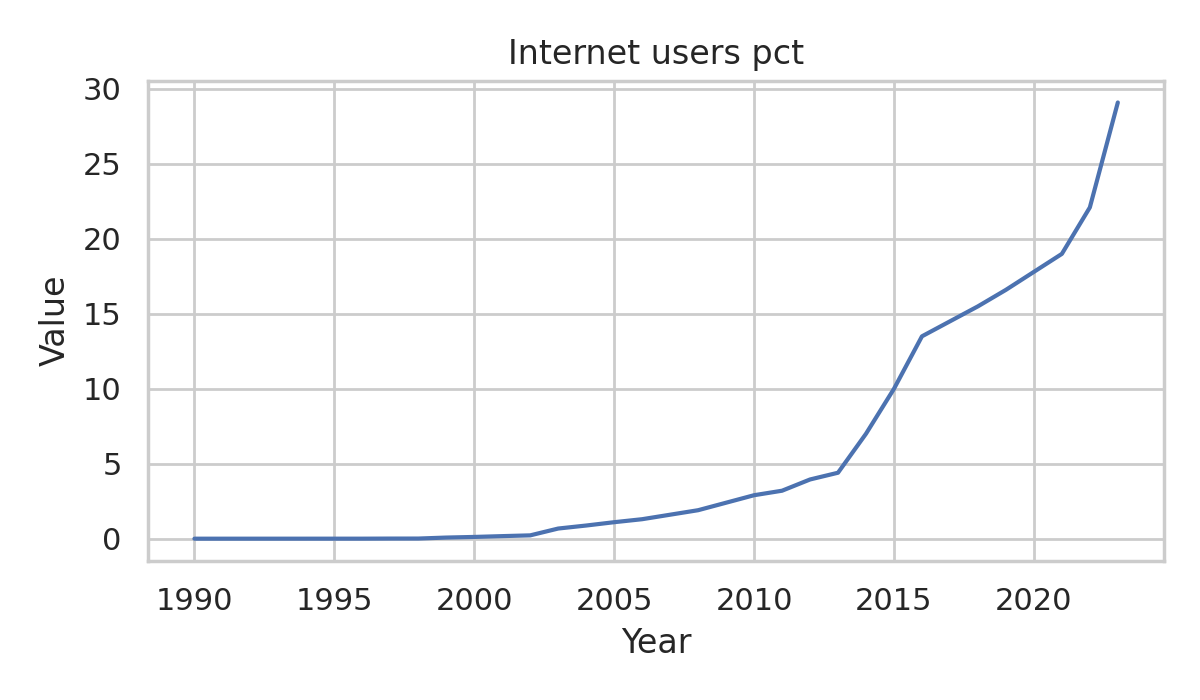
\includegraphics[width=.7\\textwidth]{figures/wb_internet_users.png}
  \\caption{Individuals using the Internet (\\% of population), Tanzania}
\\end{figure}
\\begin{figure}[!ht]
  \\centering
  \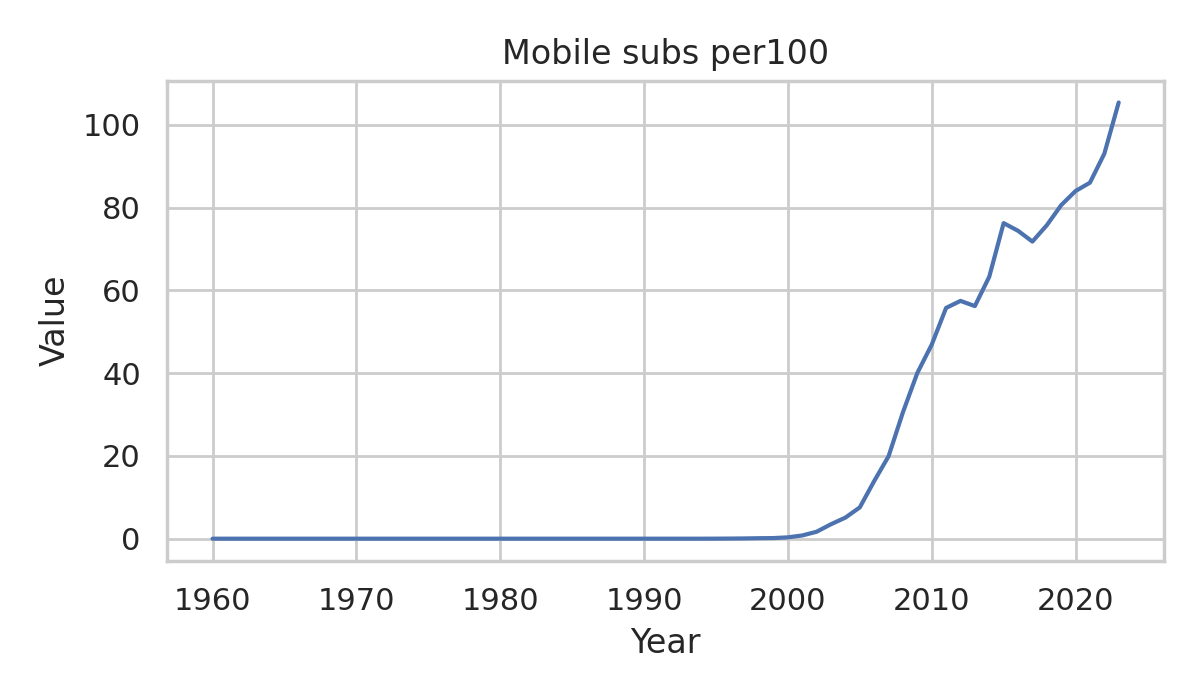
\includegraphics[width=.7\\textwidth]{figures/wb_mobile_subs.png}
  \\caption{Mobile cellular subscriptions (per 100 people), Tanzania}
\\end{figure}
\section{Rationale for Tanzania}
Unique growth trajectory and infrastructural deficits present a pertinent testbed for OI.
